%%____________________________________________________________________________||
\clearpage
\section{Systematic uncertainties in the transfer factors}
\label{sec:systematics}

This section addresses the estimation of systematic uncertainties
affecting the transfer factors (equation~\ref{equ:tf-ratio})
for non-multijet backgrounds. 
These uncertainties will be often referred to as \textit{``normalisation uncertainties''}, 
as opposed to the \textit{``template uncertainties''} described in Sec.~\ref{sec:syst-on-shape}. 
The former affect the total number of events in each (\njet,~\nb,~\scalht) bin (integrating over \mht), 
while the latter encode the limited knowledge on how these events distribute in the \mht dimension.

Two approaches are used to derive uncertainties from specific sources:
one is based on variations in simulation (Sec.~\ref{sec:mc-variations}), the other makes use of control samples in data (Sec.~\ref{sec:closure-tests}).
Each systematic source considered in the analysis is described below, 
together with the method used to derive the corresponding uncertainties and the correlation model. 
A summary of the all the uncertainties is given in Tab.~\ref{tab:systs}.

%%%%%%%%%%%%%%%%%%%%%%%%%%%%%%%%%%%%%%%%%%%%%%%%%%%%%%%%%%%%%%%
% MC-based systematics
%%%%%%%%%%%%%%%%%%%%%%%%%%%%%%%%%%%%%%%%%%%%%%%%%%%%%%%%%%%%%%%
\subsection{Systematic variations in simulation}
\label{sec:mc-variations}

A set of corrections are applied to the MC samples in order to improve the modelling 
of detector effects (b-tagging efficiency, jet energy response, etc.) 
as well as the simulation of the kinematics of certain processes (top $p_{T}$). 
These corrections are described in Sec.~\ref{sec:datasets}. \\
In this section the effect of varying these corrections within their uncertainties is 
presented, focusing on the relative change in the 4 type of transfer factors which are of interest 
for the background prediction, namely: $\mj \rightarrow (\znunu)$,
$\mmj \rightarrow (\znunu)$, $\gj \rightarrow (\znunu)$ and $\mj
\rightarrow \mathrm{\ttbar+W}$. 
The binning of the analysis is chosen in order to minimise the impact of 
these systematic sources, which are expected to be sub-dominant. 
However, they are propagated to the final results, taking into account
correlations and bin migration effects. 
The magnitude of the uncertainties are summarised in Table~\ref{tab:systs} at
the end of this section. 

All figures referenced in this sub-section can be found in Appendix~\ref{app:systematics}.

\subsubsection*{Jet energy scale}
\label{sec:tfSyst_jec}
The effect of varying the jet energy scale in
the \mj and \mmj control regions is investigated.  The energies of
jets used in the analysis are corrected as a function of their \pt and
$\eta$ via the procedure recommended by the JetMET POG. These
corrections have an associated uncertainty, which is propagated through the analysis. 
As the \scalht and jet multiplicity binning is mirrored in signal and control regions, 
the effect of jet energy scale on the transfer factor is expected to be small. 
However, the jet energy scale can still have an
effect due to jets moving in and out acceptance (above and below
$40\gev$). The relative change in the transfer factors is presented as a function of \scalht and jet category 
in Fig. ~\ref{fig:tfSyst_jec_muToZinv}-\ref{fig:tfSyst_jec_muToTtw}.
The changes are typically in the range of $1-5\%$.

\subsubsection*{B-tagging efficiency}
\label{sec:tfSyst_btag}

Scale factors provided by the BTV POG are applied to the MC samples
to correct for differences in the b-tagging efficiencies and 
misidentifications between simulation and data. 
The method employed is based on simple event reweighting as described in
Ref.~\cite{btagSFMethods}. 
Events are reweighted according to the probability of obtaining a particular jet configuration in data
and simulation, as determined by the b-tagging efficiencies computed
in the MC samples and the scale factors measured in data.
Since no extrapolation is performed in the background prediction across different 
\nb multiplicities, the analysis is expected to be robust against variations in the 
b-tagging efficiency. 
To test this effect the change in the transfer factors is measured
by varying the scale factors within their uncertainties. The scale factors
associated with b and c jets are varied together (since their measurements are
correlated), while those associated with light jets are varied separately.
The relative change in the transfer factors is presented as a function of \scalht and jet category 
in Fig. ~\ref{fig:tfSyst_bsf_muToZinv}-\ref{fig:tfSyst_bsfl_muToTtw}.
They are typically in the range of $1-3\%$.

\subsubsection*{Lepton and photon trigger/identification/isolation efficiency}
\label{sec:leptonSyst}
Leptons out of $p_{T}$ and $\eta$ acceptance, or within detector
acceptance but not identified properly by lepton identification or isolation
requirements contribute to the so-called ``lost-lepton background'', 
which mainly stem from W and \ttbar events. 
The fraction of events with leptons out of acceptance (\flepAccep)
is calculated from generator truth level information for each MC
sample. Differences in efficiencies between data and simulation are
accounted for with data/MC scale
factors for trigger, lepton identification and isolation~\cite{twiki-leptonSF}, 
and change the lost lepton background in the signal region and yields in 
muon control regions simultaneously.

The effect of lepton reconstruction on the lost lepton background
can be summarised in the following expressions respectively:
\begin{equation}
    \label{eq:lostLepSR}
    \sum_{sample} [ R_{sample} \times \flepAccep \times N^{GEN}_{sample} \times ( 1 - \epsilon_{Loose} ) + ( 1 - \flepAccep ) \times N^{GEN}_{sample} ]
\end{equation}
\begin{equation}
    \label{eq:lostLepCR}
    \sum_{sample} N^{GEN}_{sample} \times \epsilon_{Tight} \times R_{sample}
\end{equation}
where $R_{sample}$ is the cross section reweighting factor for each sample, 
$N^{GEN}_{sample}$ is the total MC events for the category, $\epsilon_{Tight}$
and $\epsilon_{Loose}$ are the lepton efficiency for Tight and Loose working 
point. For the numerator, full
signal selection except the lepton veto to mimic signal region phase space as
closely as possible. For the denominator, the full selection for the \mj 
control sample is applied.

The systematic variations on the signal region and control region are computed 
by varying the lepton scale factor
up and down according to each source of uncertainty.
Data/MC lepton scale factors have negligible statistical uncertainties. 
The procedure is repeated separately for muons and
electrons.
A log-normal systematic uncertainty of 5\% is assigned to $\mathrm{tt+W}$ in the signal region, 
and one with 2\% to the control region. The two systematics are taken to be anti-correlated 
with each other.

Finally, the $\eta$-dependent muon tracking scale factors provided by the muon 
POG to cover the effect of HIP inefficiencies have been applied and their 
uncertainties taken into consideration. Their effect on the transfer factors
is found to be less than 1\%.

\subsubsection*{Lepton Acceptance}
Theoretical uncertainties from parton distribution function and factorisation can 
introduce systematic uncertaintes on lepton acceptance, i.e. the fraction of leptons out 
of $p_{T}$ or $\eta$ range. The effect can then be parametrized with the variable \flepAccep 
in Section~\ref{sec:leptonSyst}
Theoretical uncertainties from parton distribution function
are varied according to the recommended prescription from PDF4LHC~\cite{PDF4LHC:2015}. The systematic variations 
are found to be less than 1\%.

\subsubsection*{Photon trigger uncertainty}
\label{sec:tfSyst_photonTrigger}

Variations in the trigger weight for the signal region are studied. A conservative systematic
uncertainty on this correction is taken as the size of the inefficiency. 
The relative change in the \gj transfer factor is presented in Fig.~\ref{fig:tfSyst_photonTrigger_gjToZinv}
variation is typically in the range $0-3\%$.

\subsubsection*{Signal trigger uncertainty}
\label{sec:tfSyst_trigger}

Variations in the trigger weight for the signal region are studied. A systematic is taken
as the difference in the efficiency measured using muon and electron reference triggers.
The relative change in the transfer factors is typically in the range
$1-7\%$, as presented in Figs.
~\ref{fig:tfSyst_trigger_muToZinv}-\ref{fig:tfSyst_trigger_muToTtw}, 

%\subsubsection*{Top $p_T$ reweighting}
%\label{sec:tfSyst_topPt}
%
%Variations in the reweighting of top $p_{T}$ distribution, as first outlined in 
%Sec.~\ref{sec:SMxs}, are studied. A conservative systematic
%uncertainty on this correction is taken as the size of the correction itself. 
%The relative change in transfer factors is presented in Fig.
%~\ref{fig:tfSyst_topPt_muToZinv}-\ref{fig:tfSyst_topPt_muToTtw}. The
%variation is typically in the range $0-15\%$.

%\subsubsection*{QCD contamination}
%\label{sec:tfSyst_qcdCont}
%
%A check has also been performed on the systematic effect on the
%background prediction due to QCD contamination in the control samples,
%which has been found to be at the ~5\% level for the \gj
%control region. Applying an arbitrarily large variation of $\pm
%100\%$ on the number of Monte Carlo QCD events leads to a systematic
%variation on the transfer factors of at most 5\% in the majority of bins.
%This preliminary study suggests that effect from QCD
%contamination in the \gj control region is small compared 
%to the total uncertainty assigned to transfer factors. 
%This systematic source is covered in the data-driven study  
%using the photon control region, described in Sec. ~\ref{sec:tfSyst_ZGratio}.

\subsubsection*{PU reweighting}
\label{sec:tfSyst_pu}

Events in simulation are reweighted in order to match the distribution 
of the primary vertex multiplicity observed in data, as described in Sec. ~\ref{sec:pileup-reweighting}.
A systematic uncertainty is derived by propagating 
the 5\% uncertainty on the minimum bias cross section used in the reweighting procedure. 
The relative change in the transfer factors under this variation is
small (\~1-7\%)
and shown in each analysis bin in Fig. ~\ref{fig:tfSyst_pu_muToZinv}-\ref{fig:tfSyst_pu_muToTtw}.

%\clearpage
%% %%%%%%%%%%%%%%%%%%%%%%%%%%%%%%%%%%%%%%%%%%%%%%%%%%%%%%%%%%%%%%%%
%% % Closure tests
%% %%%%%%%%%%%%%%%%%%%%%%%%%%%%%%%%%%%%%%%%%%%%%%%%%%%%%%%%%%%%%%%%

\subsection{Systematics uncertainties from data-driven tests}
\label{sec:closure-tests}
This analysis aims to rely as much as possible on the data control samples
to check for sources of bias in the transfer factors due to potential limitations in
the simulation modelling. 
Therefore, along with the MC variations mentioned above, tests are performed 
in which the number of events in a given data control sample is predicted 
using events from another data control sample and the corresponding transfer factor built in MC. 
The agreement between the predicted and observed yields is
expressed as the ratio $(\nobs - \npre)/\npre$ while considering only
the statistical uncertainties on \npre and \nobs. Therefore, the level
of closure is defined by the statistical significance of a deviation
in the ratio from zero.
These tests are performed separately for each \njet category, as a function of \scalht. 
The systematic uncertainty in each \scalht bin is derived by summing in quadrature the ratio 
defined above with its statistical error, after merging the \njet categories into symmetric and asymmetric topologies. 
Pairs of \scalht bins are merged when the $\mu\mu$+jets sample is used, in order to gain statistics. 
These systematics are considered un-correlated in each \scalht bin and jet topology. 
The magnitude of the uncertainties are summarised in Table~\ref{tab:systs} at
the end of this section. 

\subsubsection*{Extrapolation in \alphat and \bdphi}
\label{sec:tfSyst_alphaT}
The modelling of the \alphat and
\bdphi extrapolations are also tested with dedicated tests in data. 
In both cases, it is checked that events with genuine \met found in the core
of the variable distribution below some threshold value can be used to
predict the events in the tail (above the same threshold value).
This is important to verify the
approach of using \mj and \mmj samples without an \alphat requirement
to make background predictions in the signal region. The tests
confront data yields in a \mj  samples with an \alphat /\bdphi
requirement against predictions determined in a \mj sample with
the \alphat /\bdphi requirement inverted. 
The contribution to the systematic error for \met extrapolation is taken
from the \alphat closure tests for bins with $\scalht<800\gev$ and from 
the \bdphi tests for bins with $\scalht>800\gev$. 

The result of these tests are shown in Figs.~\ref{fig:closureAlphaT}
and~\ref{fig:closure_bdphi} as a function of \scalht and \njet. 
The grey band is the systematic uncertainty propagated through the analysis, 
taken as un-correlated per each \scalht bin and jet topology
(symmetric/asymmetric). The systematic derived from these tests is
in the range $3-20\%$.

\subsubsection*{Modelling of the W/Z ratio}
\label{sec:tfSyst_WZratio}
To validate the use of \wmj and \ttbar dominated \mj events to predict the \znunu
background, tests are performed in data using single-muon and double-muon control regions. 
The events in the \mj control are used to predict events in the \mmj control regions, 
using transfer factors from simulation. 
These tests target the modelling of the W/Z ratio in simulation and 
also indirectly test muon acceptance effects, which 
are expected to be sub-dominant and whose uncertainties are already addressed elsewhere.

The result are shown in Fig.~\ref{fig:closureMuToMuMu} as a function of \scalht and \njet. 
The grey band is the systematic uncertainty propagated through the analysis, 
taken as un-correlated per each \scalht bin and jet topology (symmetric/asymmetric). The systematic derived from these tests is
in the range $1-12\%$.

\subsubsection*{Modelling of the W/Z acceptance due to polarisation effects}
\label{sec:tfSyst_Wpol}
A data-driven test is introduced to check the modelling of the W polarisation in simulation. 
In this study, carried on using events in the single-muon control region, $\mu^{+}$ events 
are used to predict $\mu^{-}$ events, using transfer factor built in MC. 
The polarisation of the W boson has an impact on the prediction 
of the \znunu background using the \mj control region, as explained in the following. 
The production mechanism of $W$ from pp
collisions means high $p_T$ $W$ bosons are predominantly left handed
\cite{WPol}.  For high $p_T$ bosons, this implies that $W^+$ decays to
the left handed neutrino along its direction of motion while the
lepton is pointing backward. The opposite behaviour is expected for
the $W^-$. The lepton is therefore more boosted (and the neutrino less
boosted) in $W^+$ decays than $W^-$ decays.  This leads to a larger
number of $W^+$ decays in the single lepton control regions (which
relies on the lepton $p_T$ for acceptance) than in the signal region
(which relies on the neutrino $p_T$ for acceptance).

The results are shown in Fig.~\ref{fig:closureMuPToMuM} as a function of \scalht and \njet. 
The grey band is the systematic uncertainty propagated through the analysis, 
taken as un-correlated per each \scalht bin and jet topology (symmetric/asymmetric). The systematic derived from these tests is
in the range $2-14\%$.

\subsubsection*{Modelling of the Z/$\gamma$ ratio}
\label{sec:tfSyst_ZGratio}
To validate the use of \gj events to predict the \znunu
background, tests are performed in data using the photon and double-muon control regions. 
The events in the \gj control are used to predict events in the \mmj control regions, 
using transfer factors from simulation. 
These tests target the modelling of the Z/$\gamma$ ratio in simulation and 
also indirectly test muon/photon acceptance effects, which, however, 
are expected to be sub-dominant and whose uncertainties are already addressed elsewhere. 

The result are shown in Fig.~\ref{fig:closurePhoToMuMu} as a function of \scalht and \njet. 
The grey band is the systematic uncertainty propagated through the analysis, 
taken as un-correlated per each \scalht bin and jet topology (symmetric/asymmetric). The systematic derived from these tests is
in the range $2-26\%$.

\subsubsection*{Modelling of the W/\ttbar admixture}
\label{sec:tfSyst_WttAd}
The $0$ b-tag $\rightarrow1$ b-tag data-driven tests in the \mj control region 
probe the sensitivity of the transfer factors to the relative
admixture of events from the $W$ + jets and \ttbar processes, 
since they utilise a W-enriched sample to predict a \ttbar-enriched sample. 
These tests indirectly probe also the modelling of the b-tagging
efficiency and the related scale factor corrections;
however, the ICHEP16 b-tag SF are applied, discussed in \ref{sec:inputs-and-updates},
thus the derived systematic is not propagated to the fit. Instead this
closure tests is inspected solely as a cross-check. 
%These tests indirectly probe also the modelling of the b-tagging efficiency, 
%although this systematic effect is expected to be smaller and is already addressed 
%by the dedicated study presented in Sec. ~\ref{sec:tfSyst_btag}.
%These tests are believed to give a conservative uncertainty, 
%as the admixture changes little between the \mj sample and the signal region, 
%given that no extrapolation between different b-tag multiplicities is performed 
%in the estimation of the background. 
%The uncertainty derived is therefore driven by the limited statistics available in the control sample. 
The result are shown in Fig.~\ref{fig:closureBTag} as a function of \scalht and \njet. 
%The grey band is the systematic uncertainty.% propagated through the analysis, 
%taken as un-correlated per each \scalht bin and jet topology (symmetric/asymmetric). The systematic derived from these tests is
%in the range $4-25\%$.

\begin{figure}[h!]
  \begin{center}
    \subfigure[]{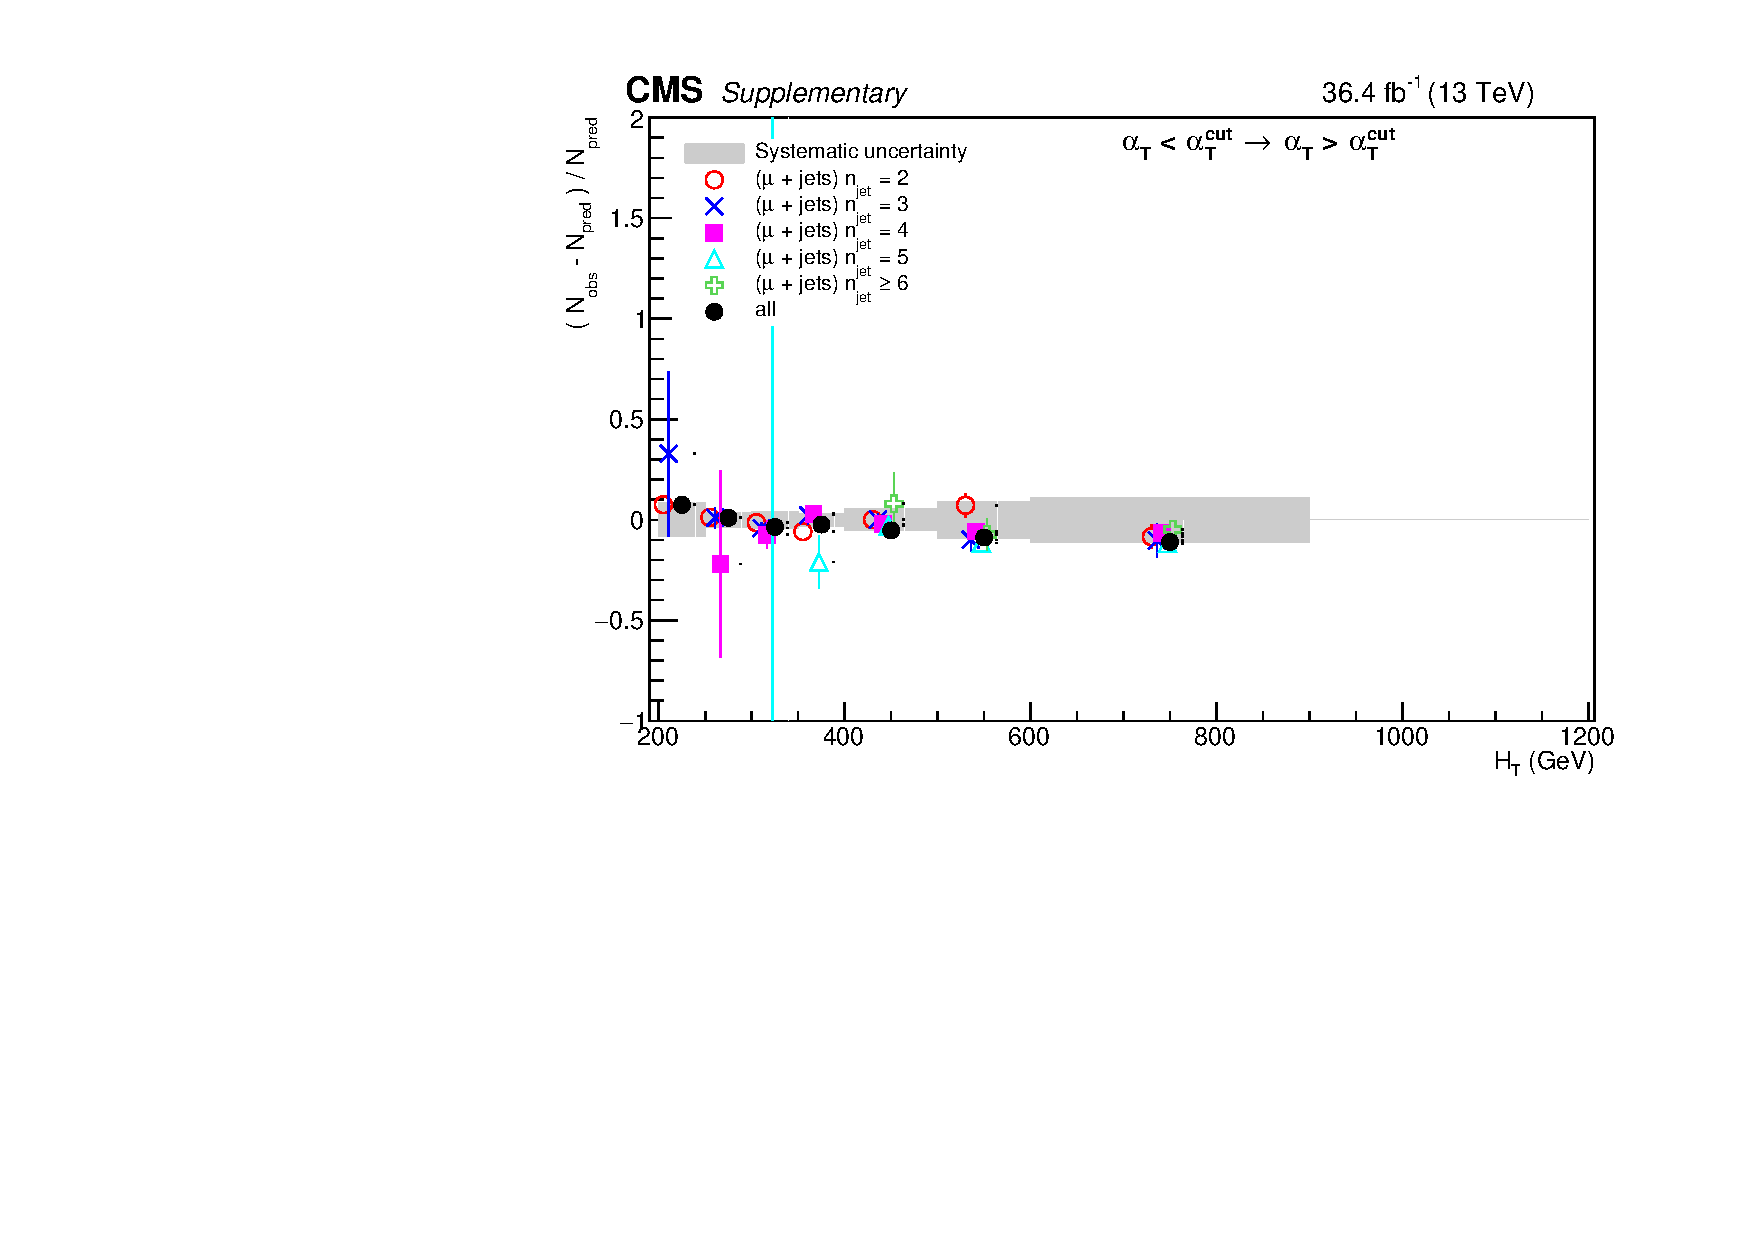
\includegraphics[width=0.5\textwidth]{figures/closureTests/alphaT_mu_sym__noFit.pdf}}
    ~~
    \subfigure[]{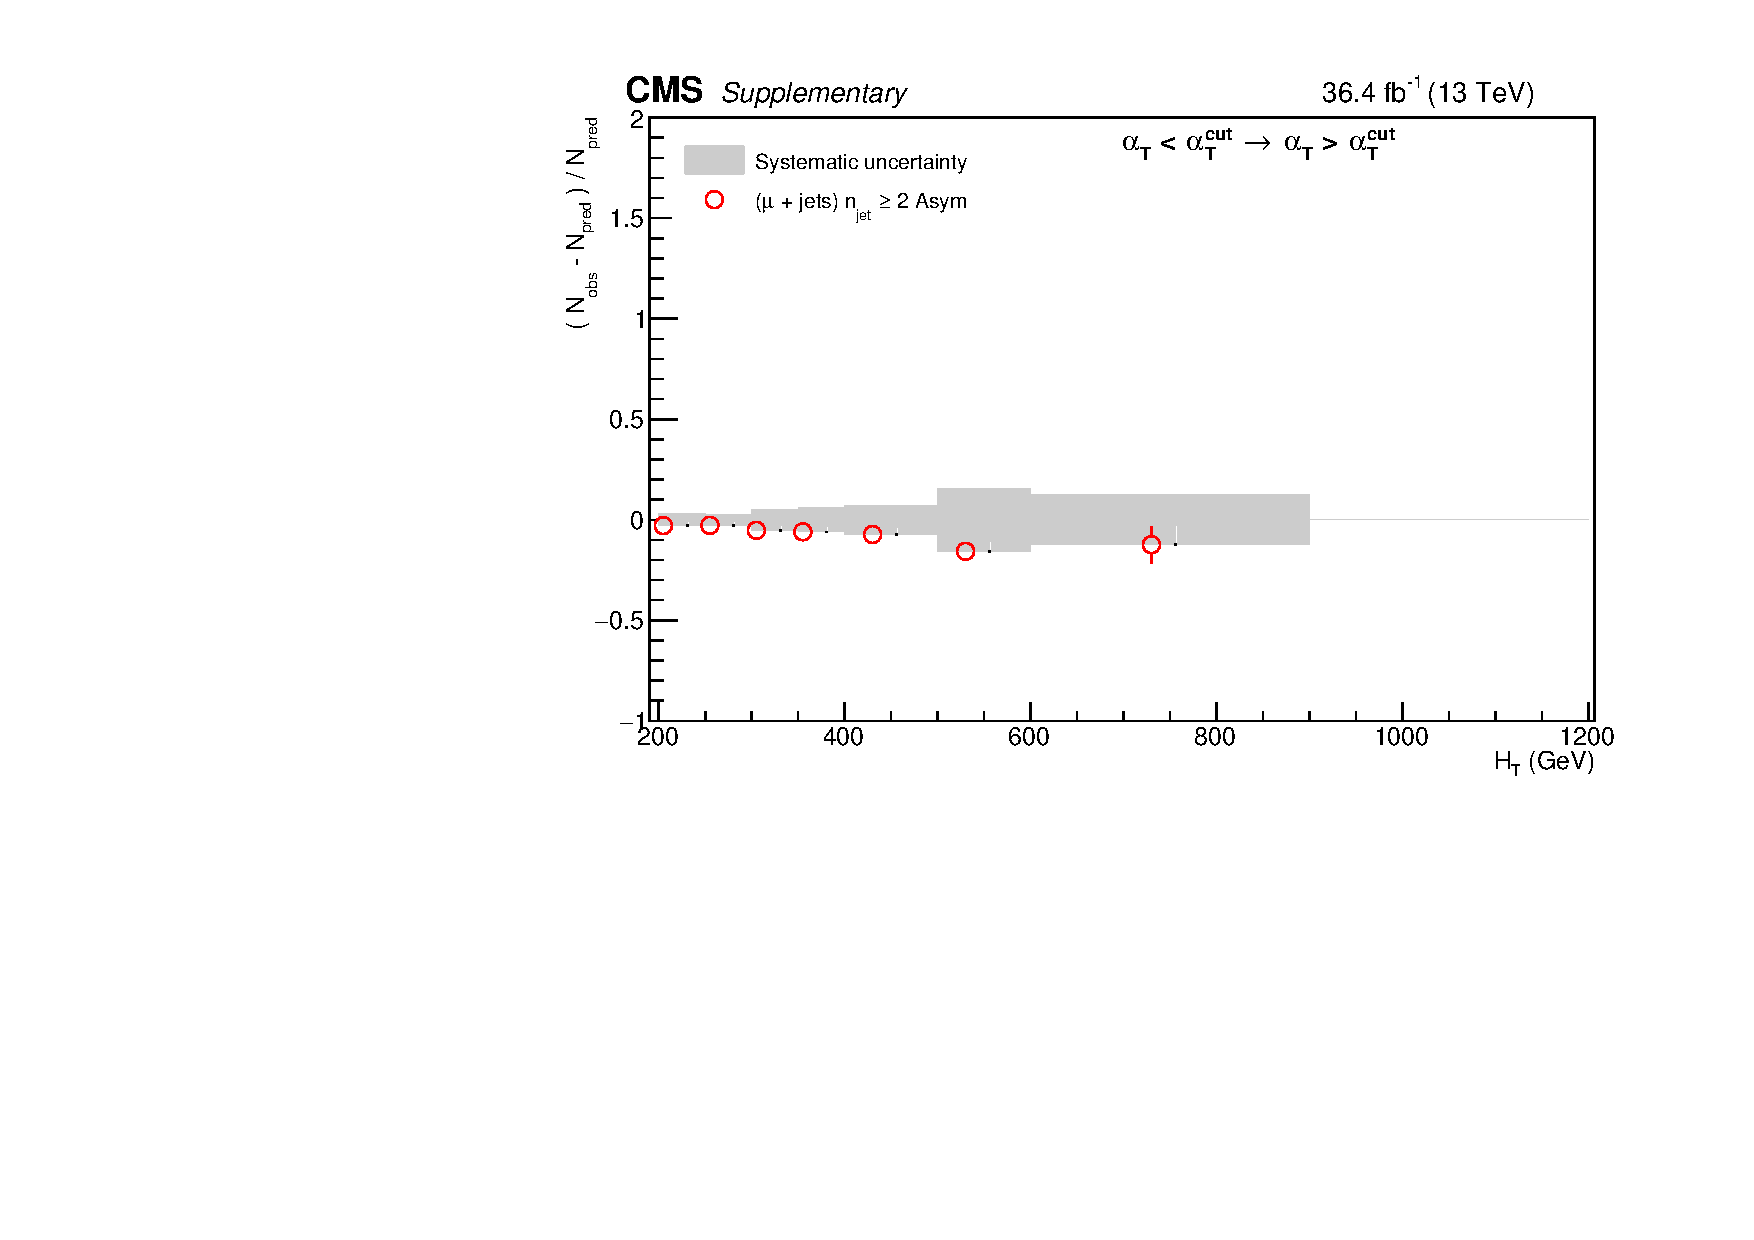
\includegraphics[width=0.5\textwidth]{figures/closureTests/alphaT_mu_asym__noFit.pdf}}
    \caption{Data-driven tests probing the \alphat extrapolation for each
      \njet category (open symbols) overlaid on top of the systematic
      uncertainty estimates used for each \scalht bin (shaded bands). 
      The symmetric (asymmetric) jet topologies are shown in the left (right) plot. 
    }
    \label{fig:closureAlphaT}
  \end{center} 
\end{figure}

\begin{figure}[h!]
  \begin{center}
    \subfigure[]{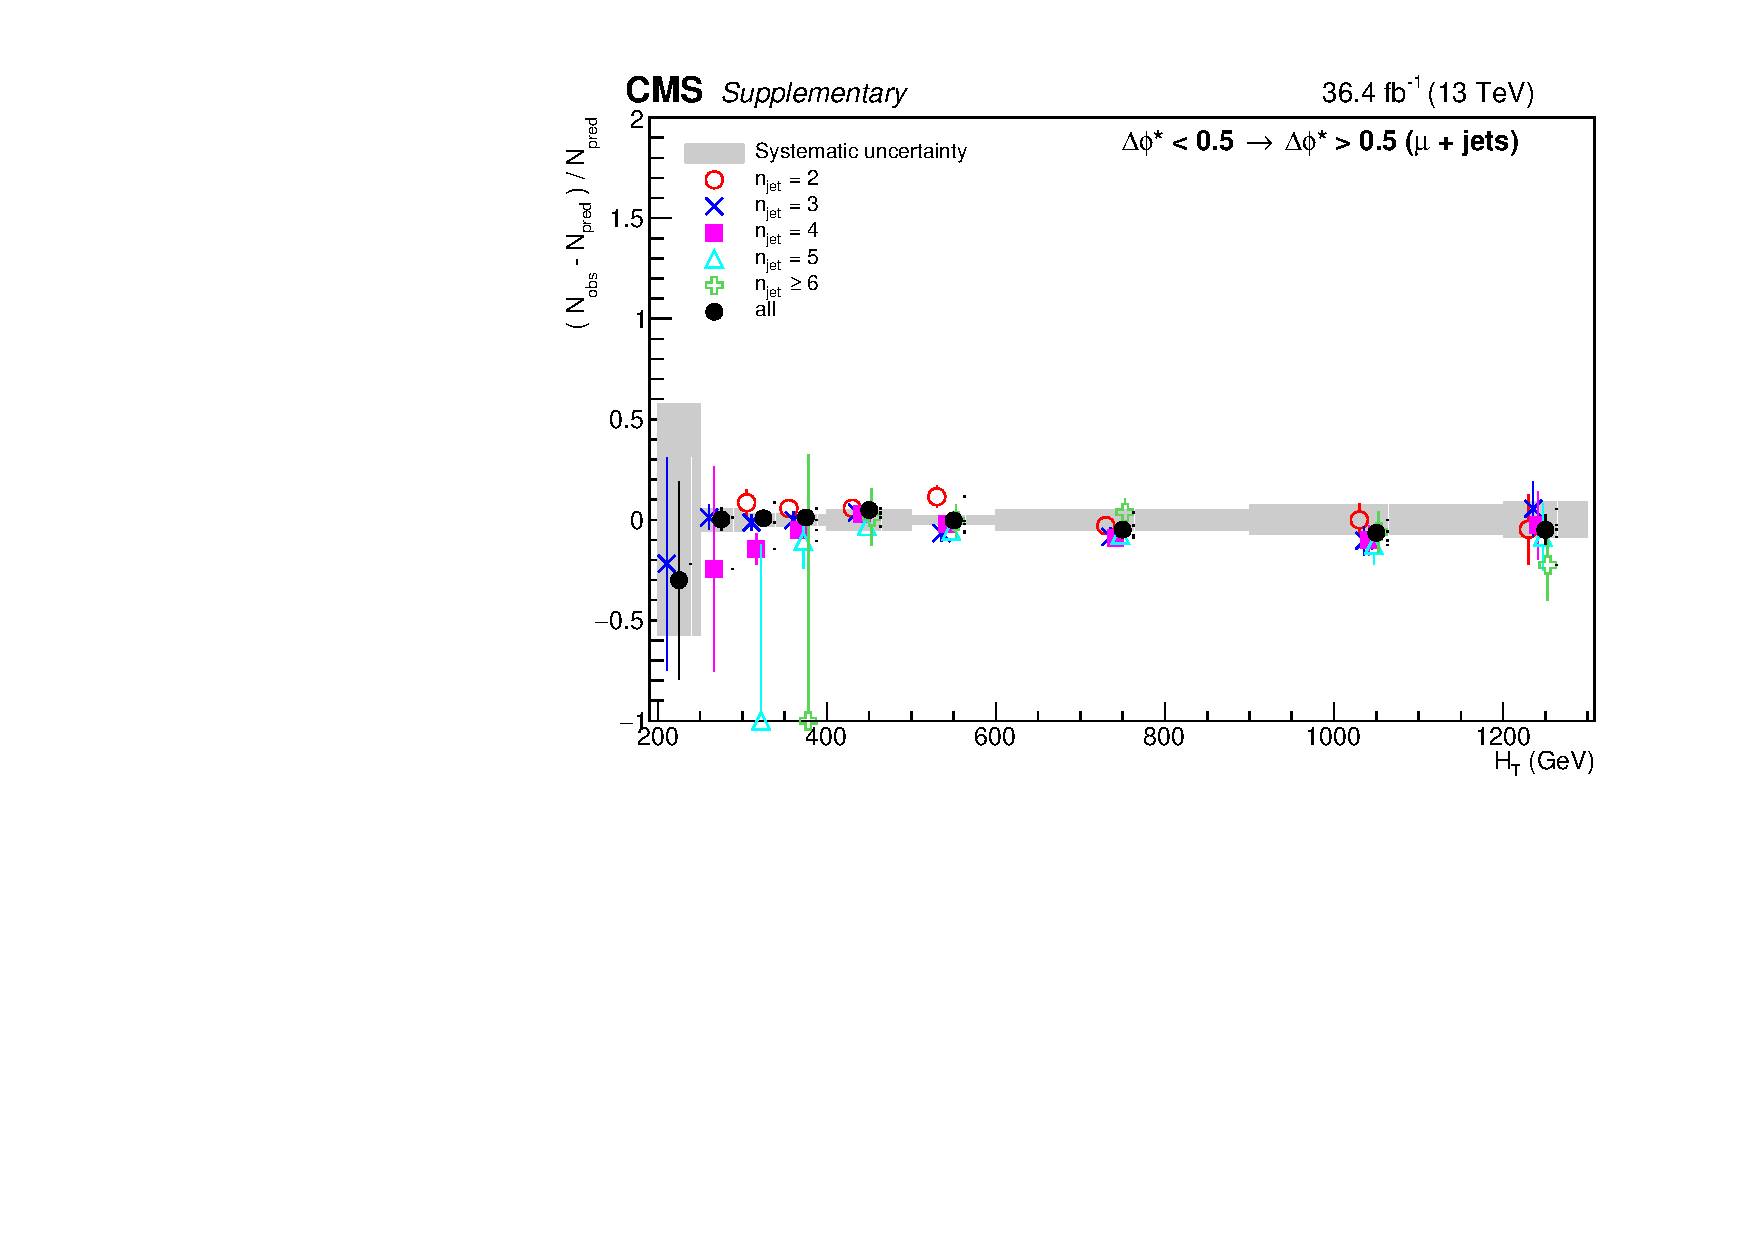
\includegraphics[width=0.5\textwidth]{figures/closureTests/bDPhi_sym__noFit.pdf}}
    ~~
    \subfigure[]{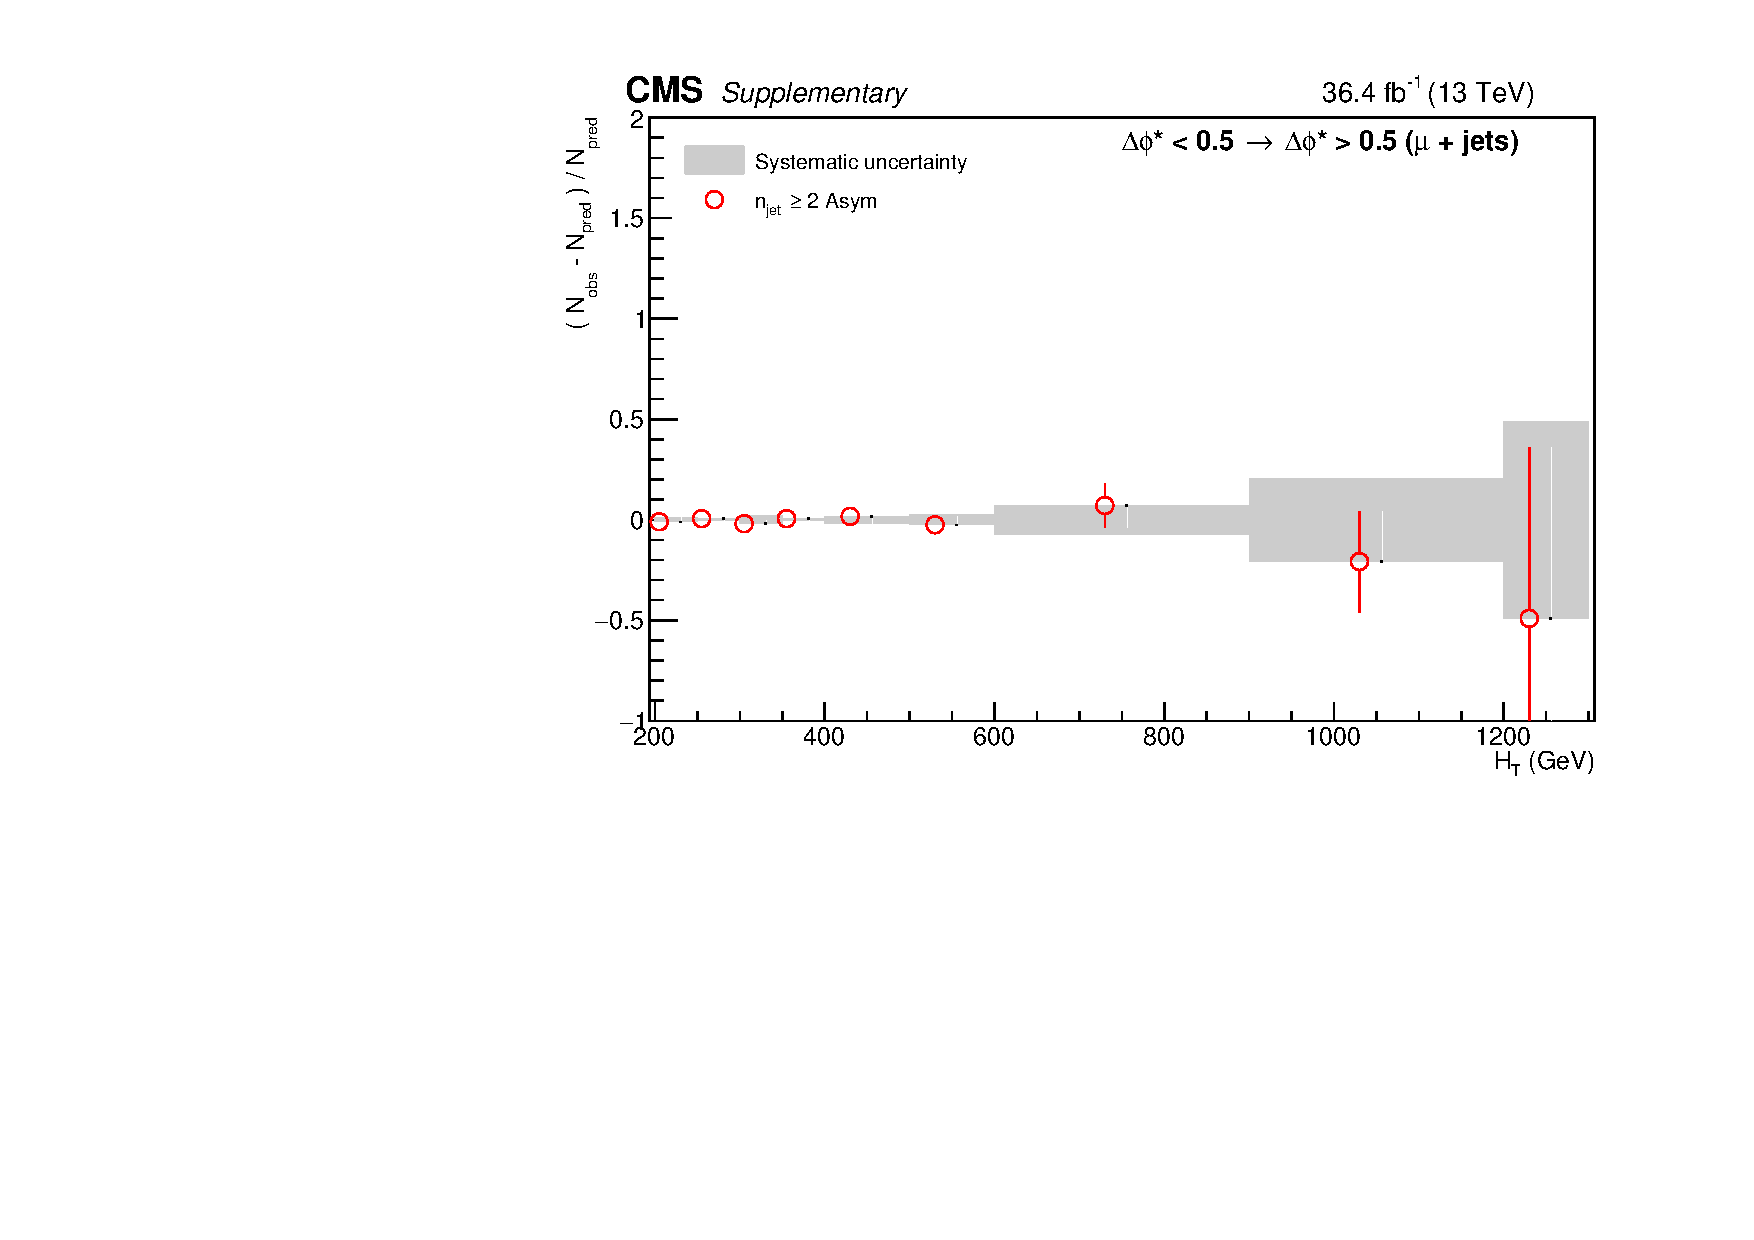
\includegraphics[width=0.5\textwidth]{figures/closureTests/bDPhi_asym__noFit.pdf}} 
    \caption{Data-driven tests probing the \bdphi extrapolation for each
      \njet category (open symbols) overlaid on top of the systematic
      uncertainty estimates used for each \scalht bin (shaded bands). 
      The symmetric (asymmetric) jet topologies are shown in the left (right) plot. 
    }
    \label{fig:closure_bdphi}
  \end{center} 
\end{figure}

\begin{figure}[h!]
  \begin{center}
    \subfigure[]{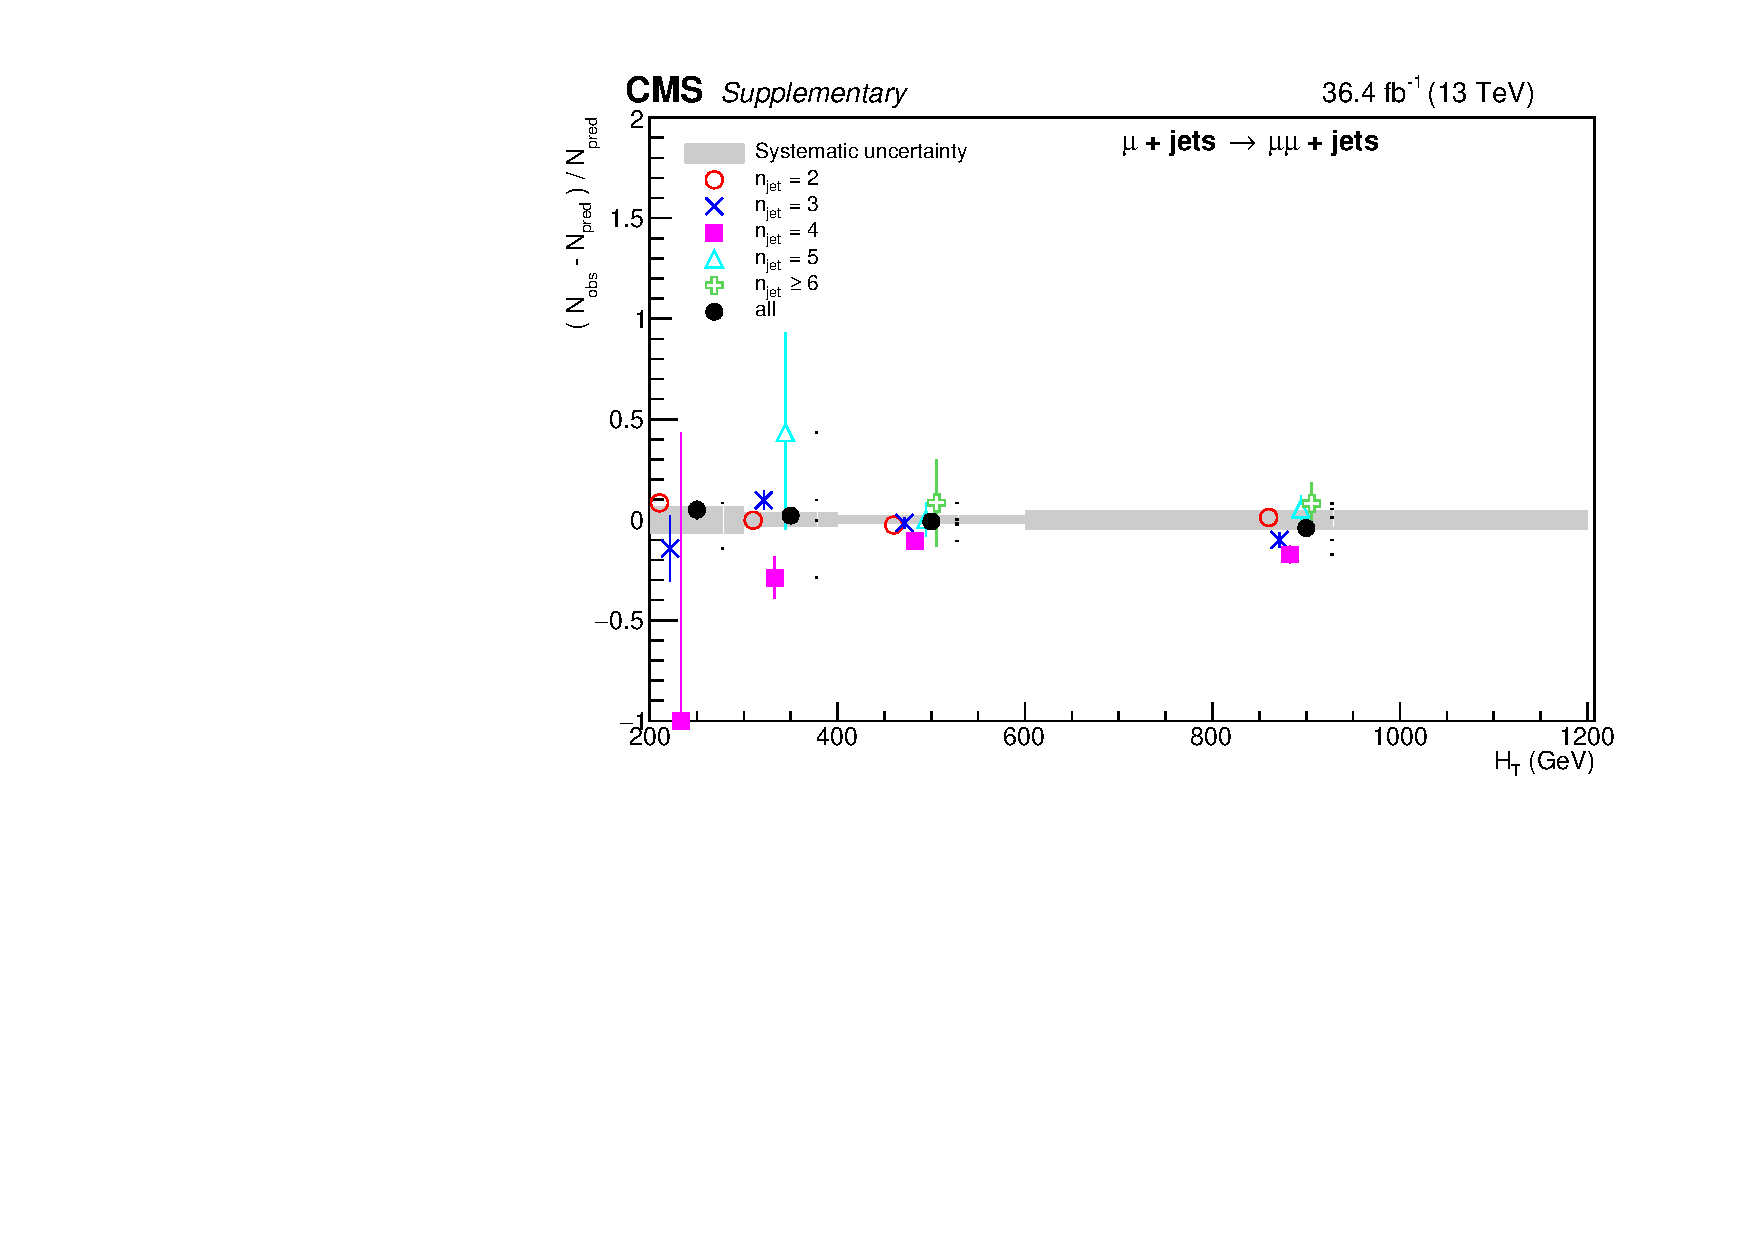
\includegraphics[width=0.5\textwidth]{figures/closureTests/mu_mumu_sym_half_noFit.pdf}}
    ~~
    \subfigure[]{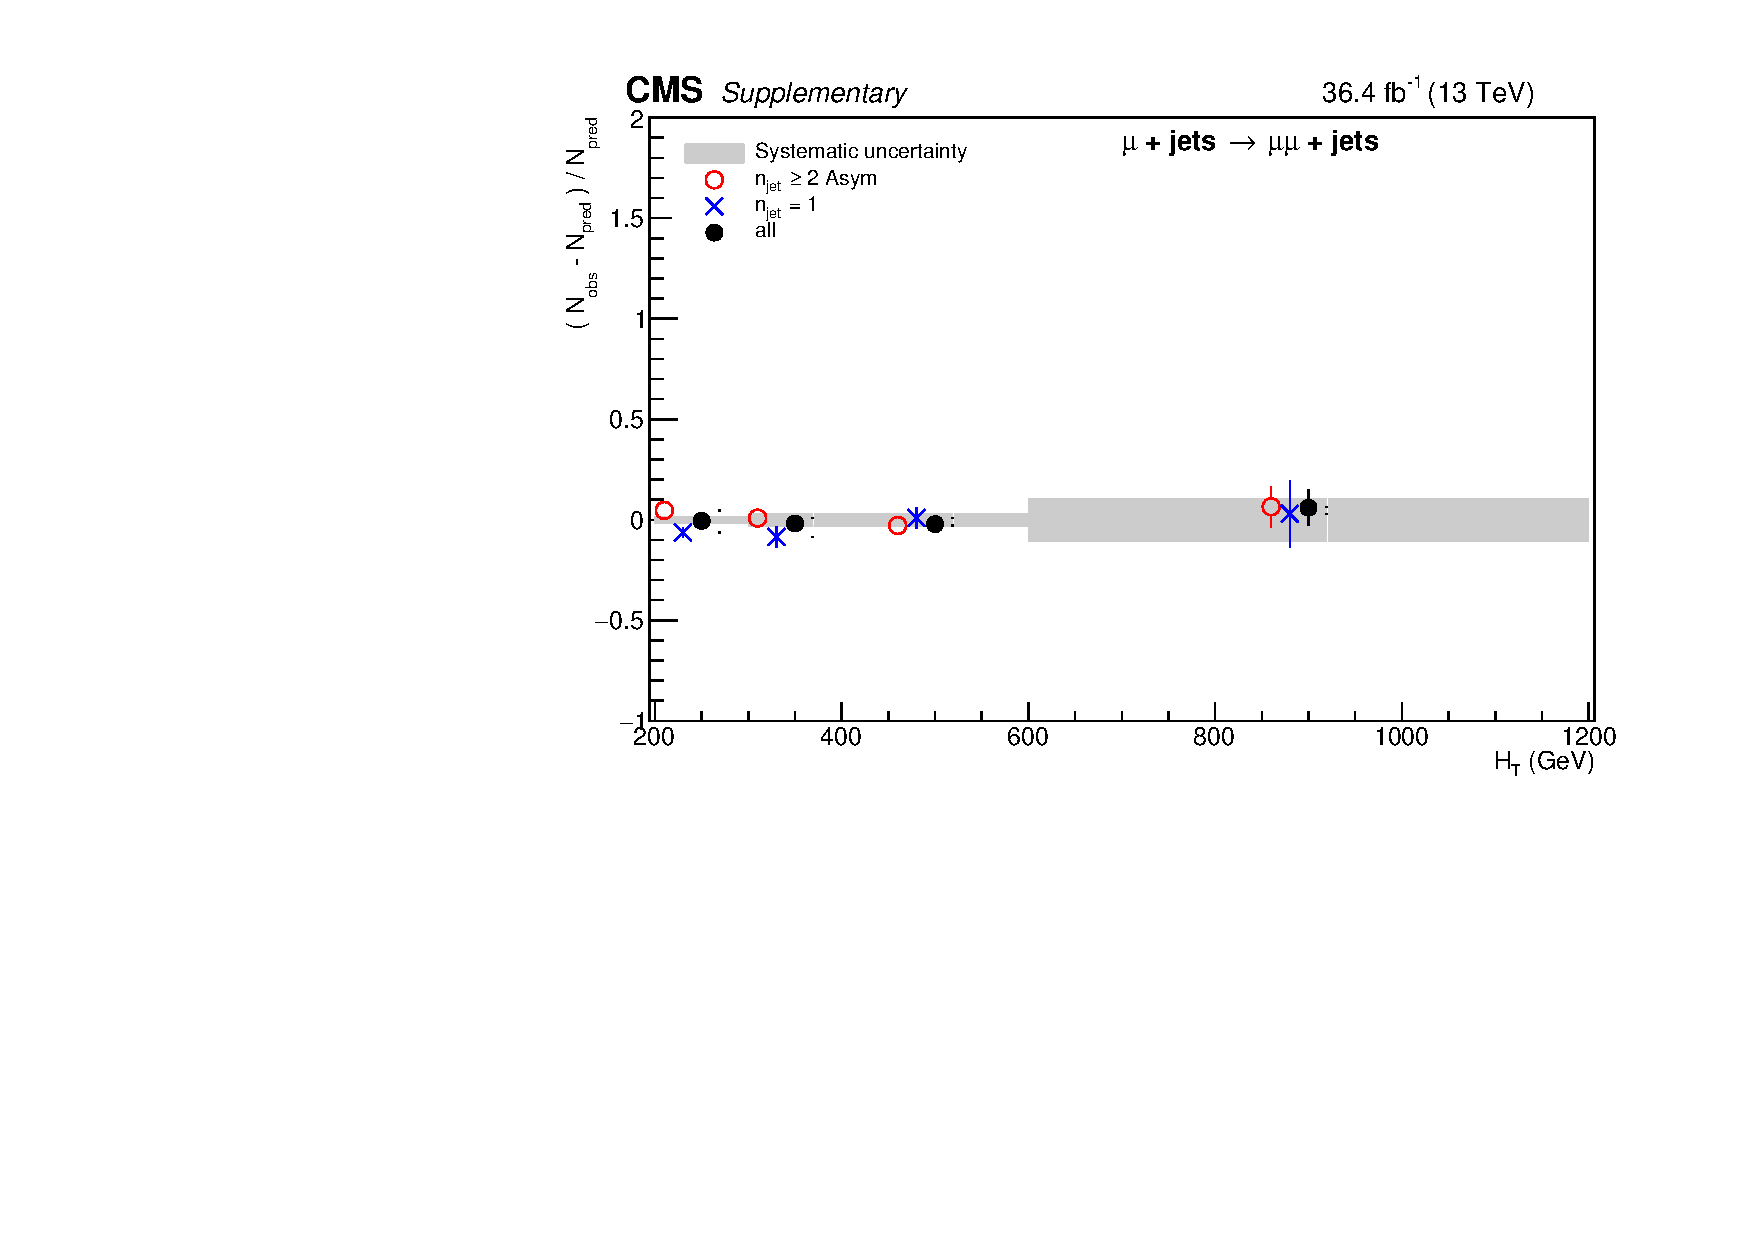
\includegraphics[width=0.5\textwidth]{figures/closureTests/mu_mumu_asym_half_noFit.pdf}} 
    \caption{Data-driven tests probing the use of the \mj control sample
      to predict the \znunu background for each
      \njet category (open symbols) overlaid on top of the systematic
      uncertainty estimates used for each \scalht bin (shaded bands).  
      The symmetric (asymmetric) jet topologies are shown in the left (right) plot. 
    }
    \label{fig:closureMuToMuMu}
  \end{center} 
\end{figure}

\begin{figure}[h!]
  \begin{center}
    \subfigure[]{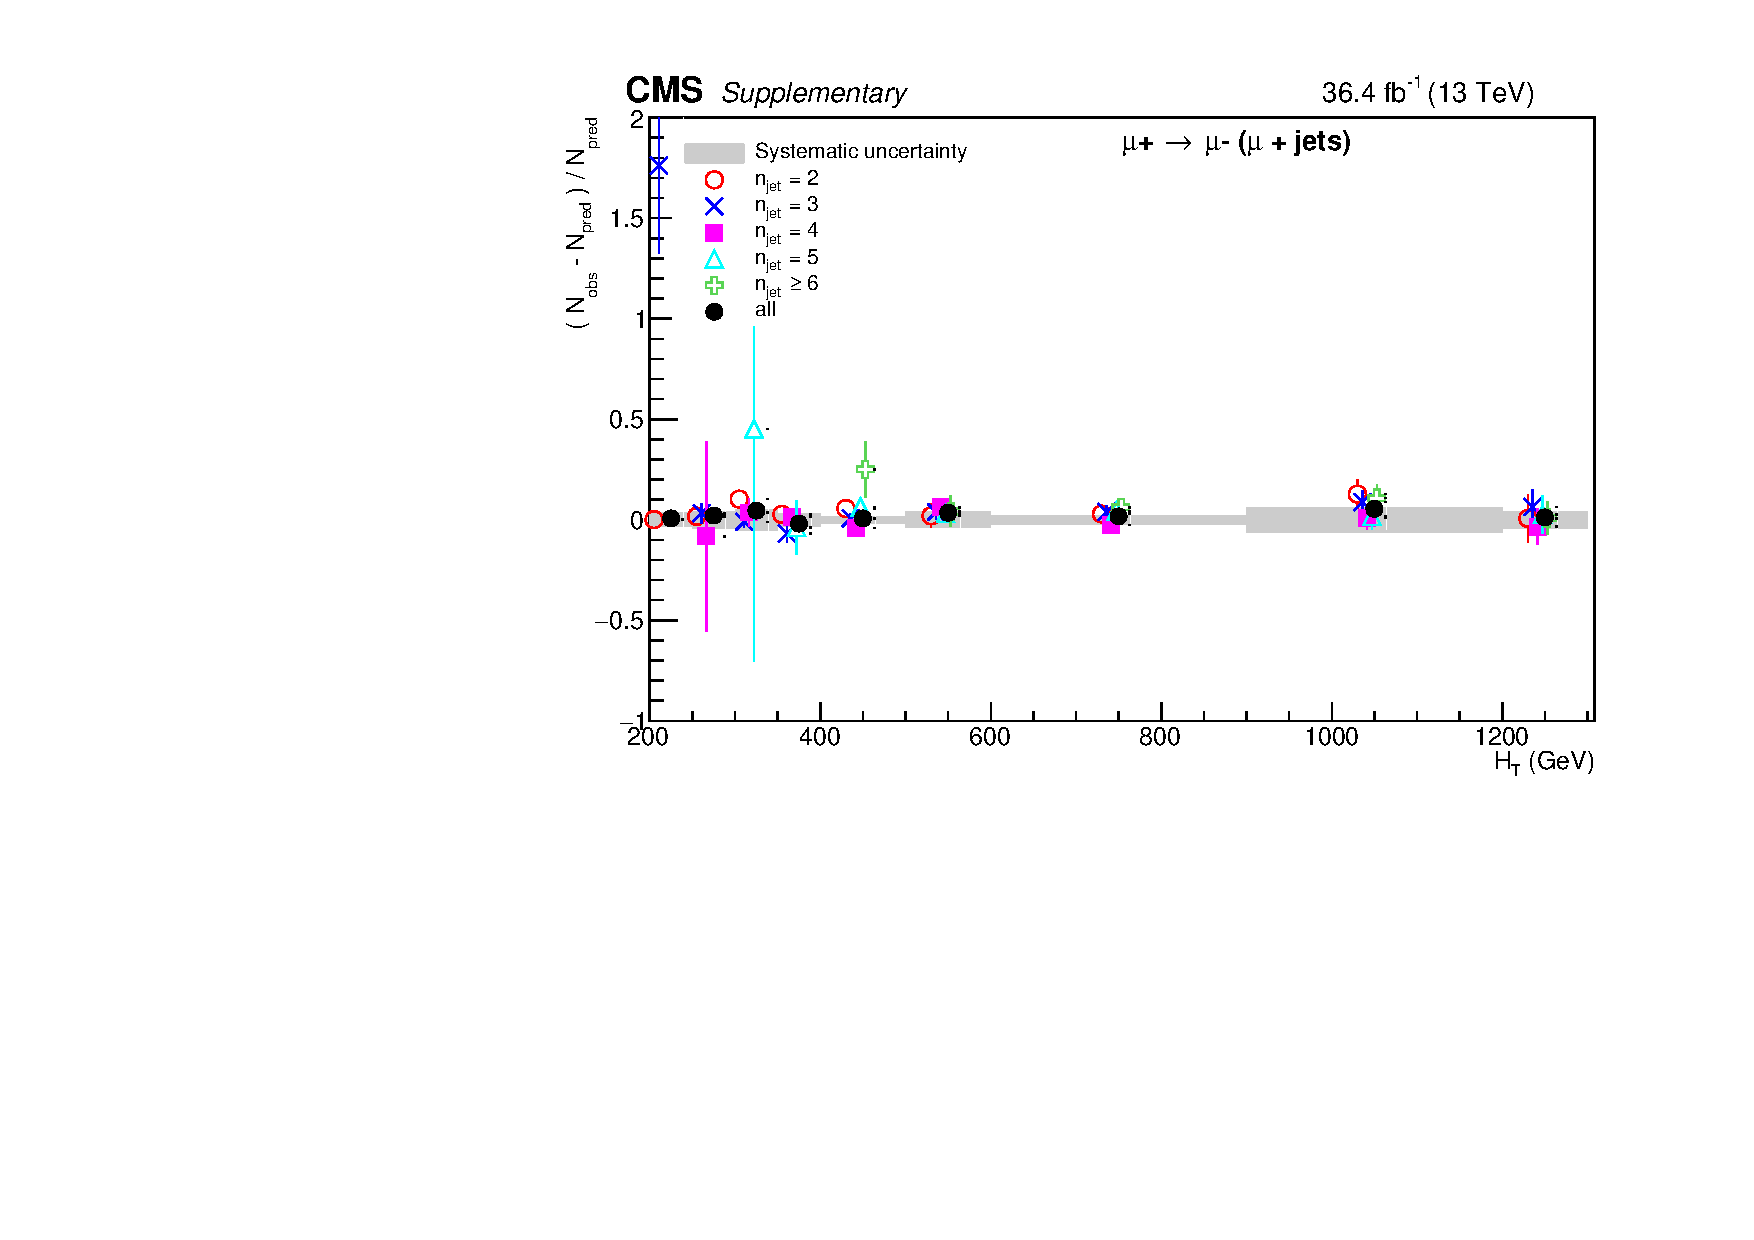
\includegraphics[width=0.5\textwidth]{figures/closureTests/muplus_muminus_sym__noFit.pdf}}
    ~~
    \subfigure[]{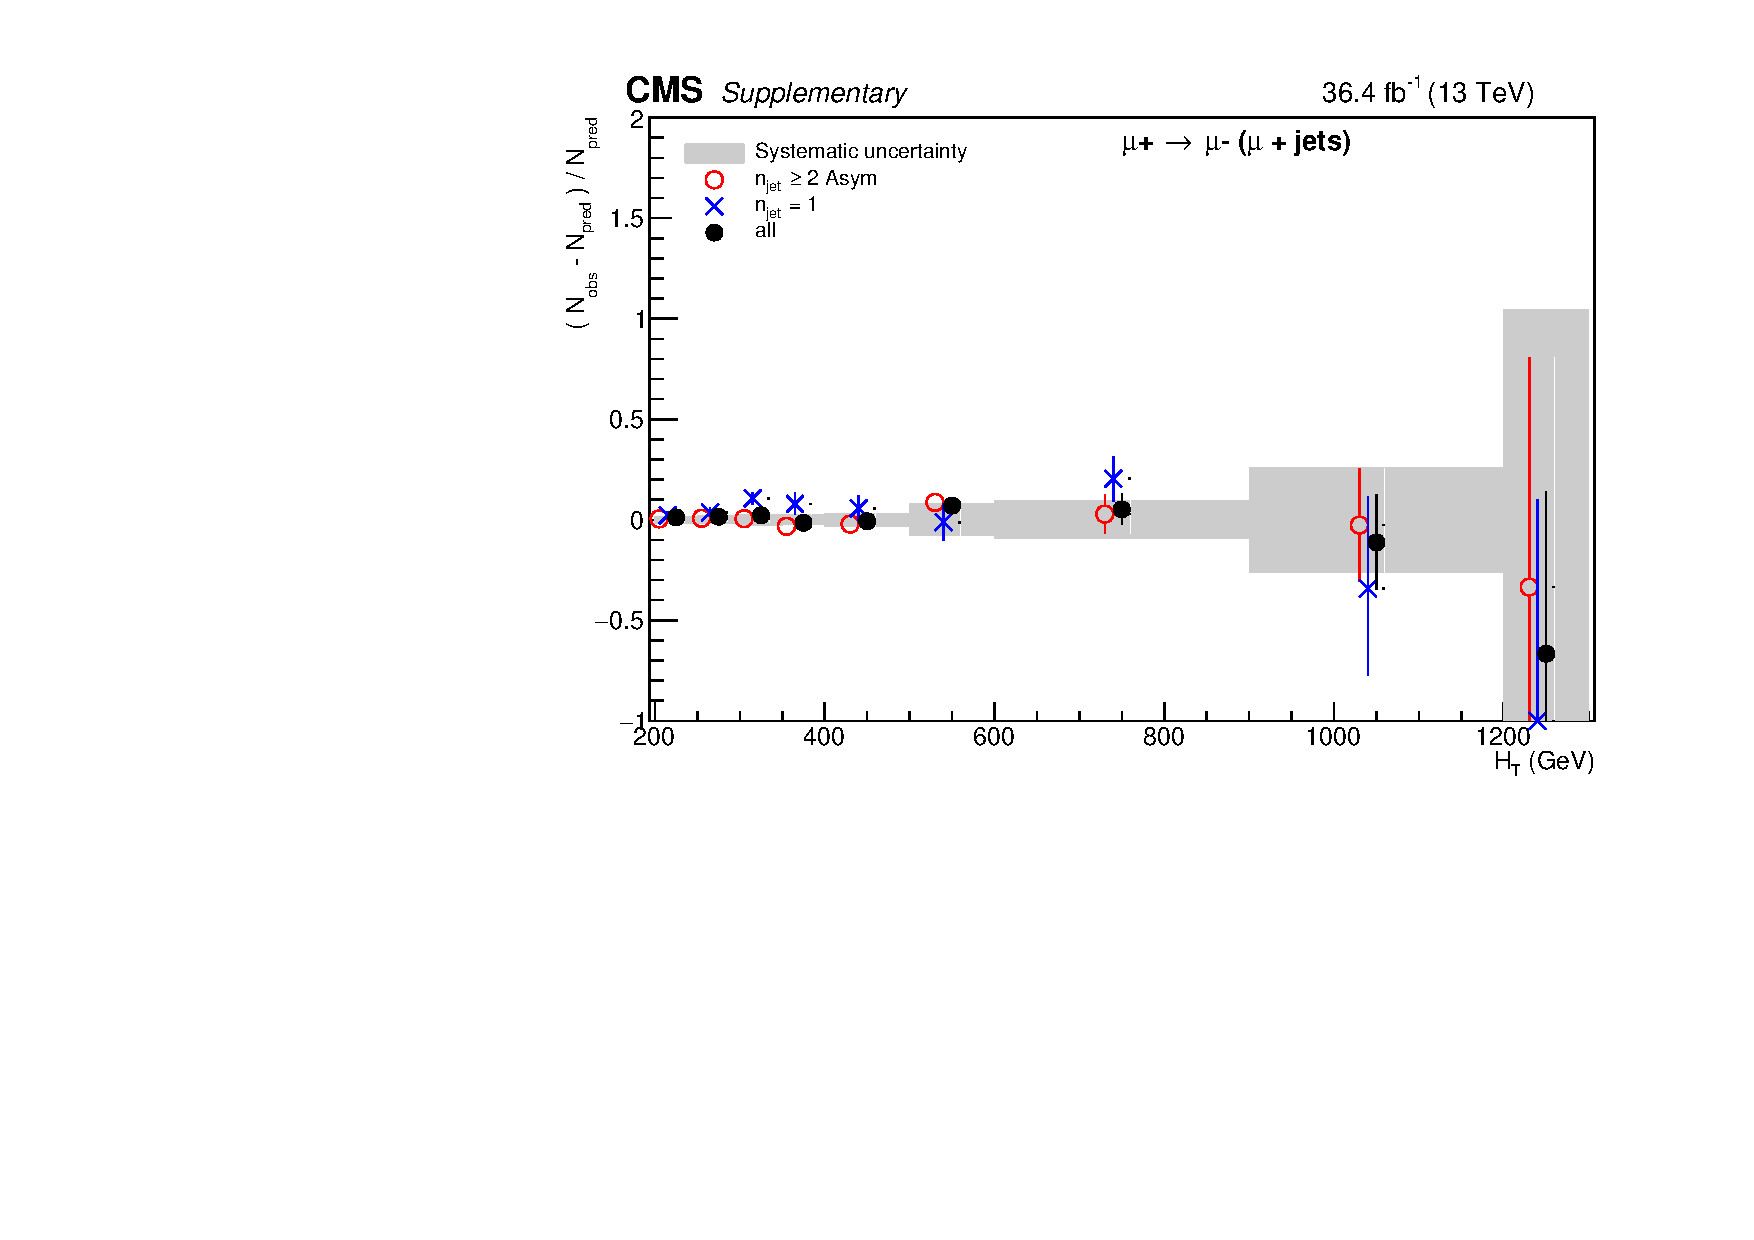
\includegraphics[width=0.5\textwidth]{figures/closureTests/muplus_muminus_asym__noFit.pdf}} 
    \caption{Data-driven tests probing the W polarisation effects. 
      These are shown for each
      \njet category (open symbols) overlaid on top of the systematic
      uncertainty estimates used for each \scalht bin
      (shaded bands). 
      The symmetric (asymmetric) jet topologies are shown in the left (right) plot.       
    }
    \label{fig:closureMuPToMuM}
  \end{center} 
\end{figure}

\begin{figure}[h!]
  \begin{center}
    \subfigure[]{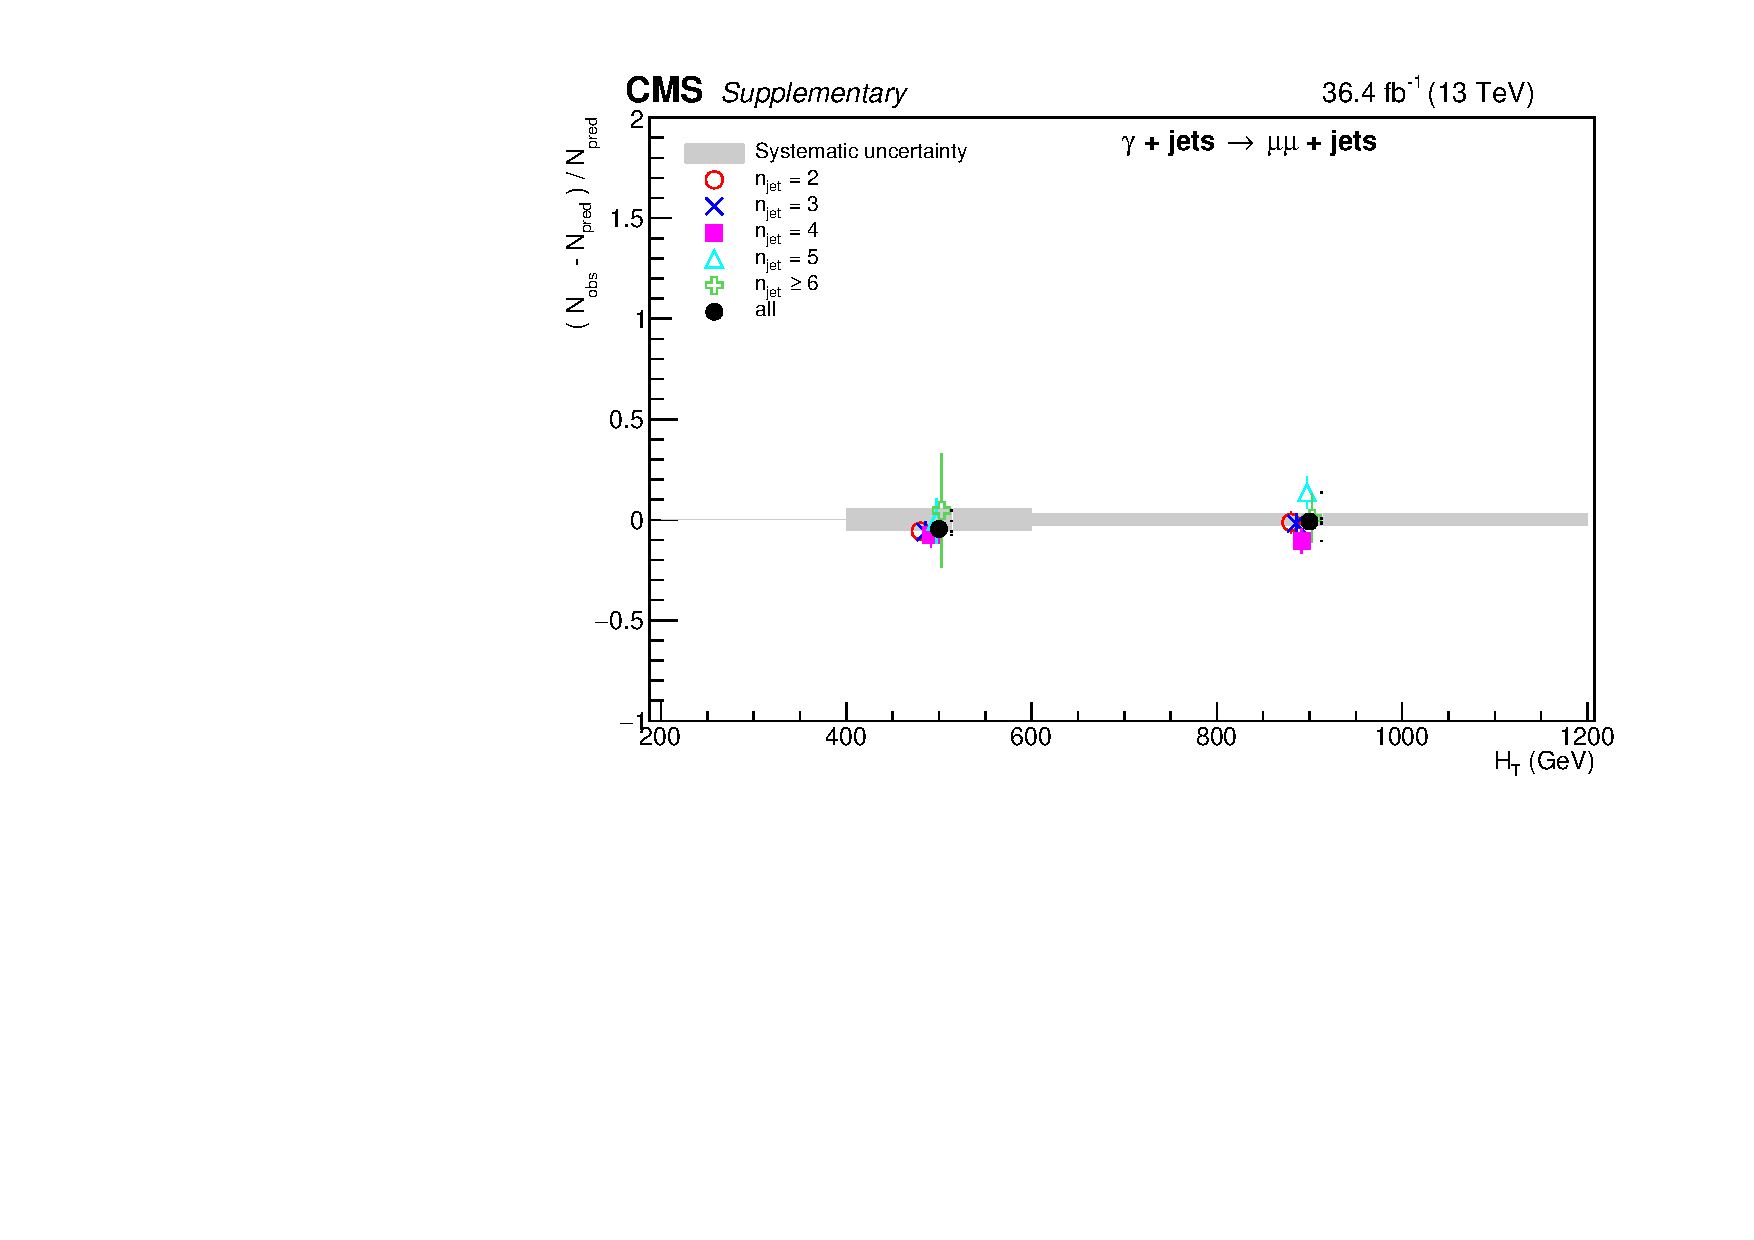
\includegraphics[width=0.5\textwidth]{figures/closureTests/phot_mumu_sym_half_noFit.pdf}}
    ~~
    \subfigure[]{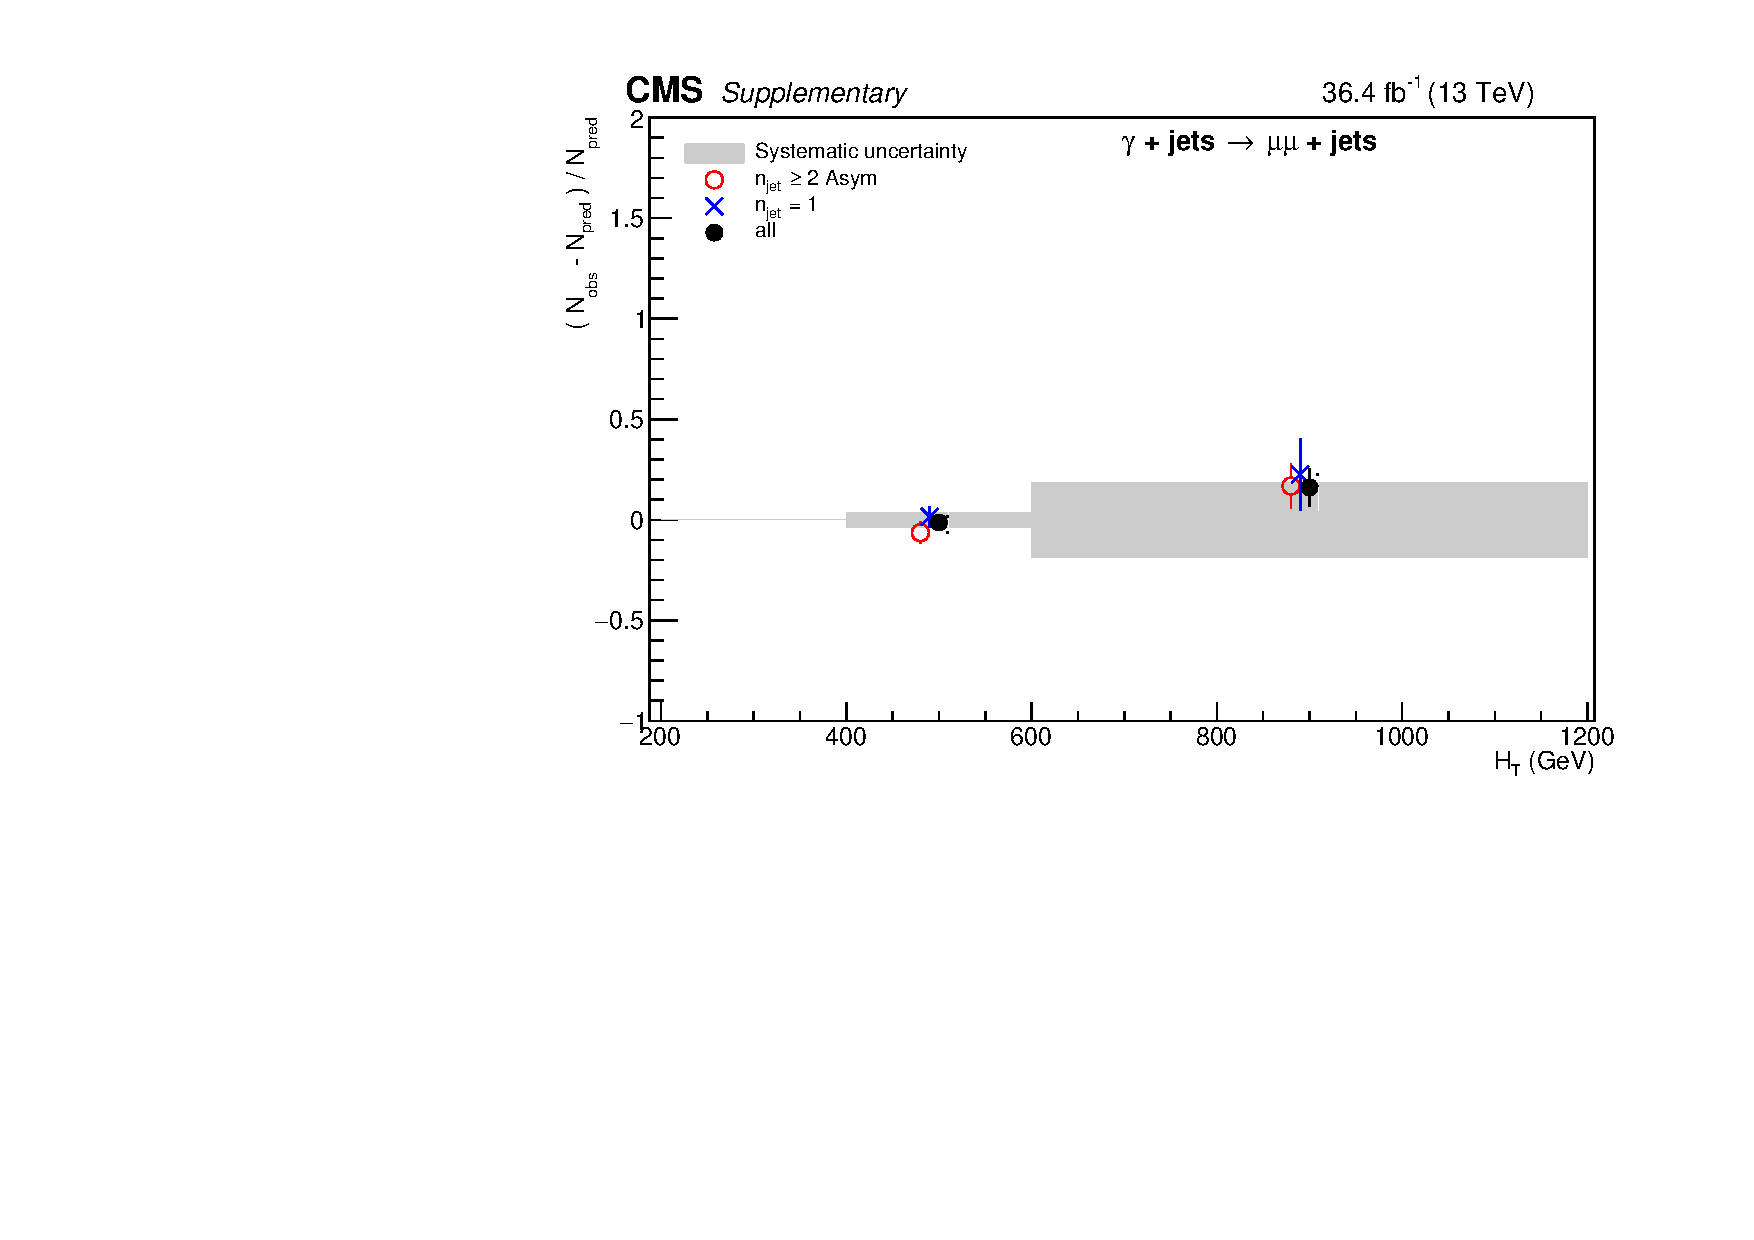
\includegraphics[width=0.5\textwidth]{figures/closureTests/phot_mumu_asym_half_noFit.pdf}} 
    \caption{Data-driven tests probing the Z/$\gamma$ ratio for each
      \njet category (open symbols) overlaid on top of the systematic
      uncertainty estimates used for each \scalht bin
      (shaded bands). 
      The symmetric (asymmetric) jet topologies are shown in the left (right) plot.      
    }
    \label{fig:closurePhoToMuMu}
  \end{center} 
\end{figure}

\begin{figure}[h!]
  \begin{center}
    \subfigure[]{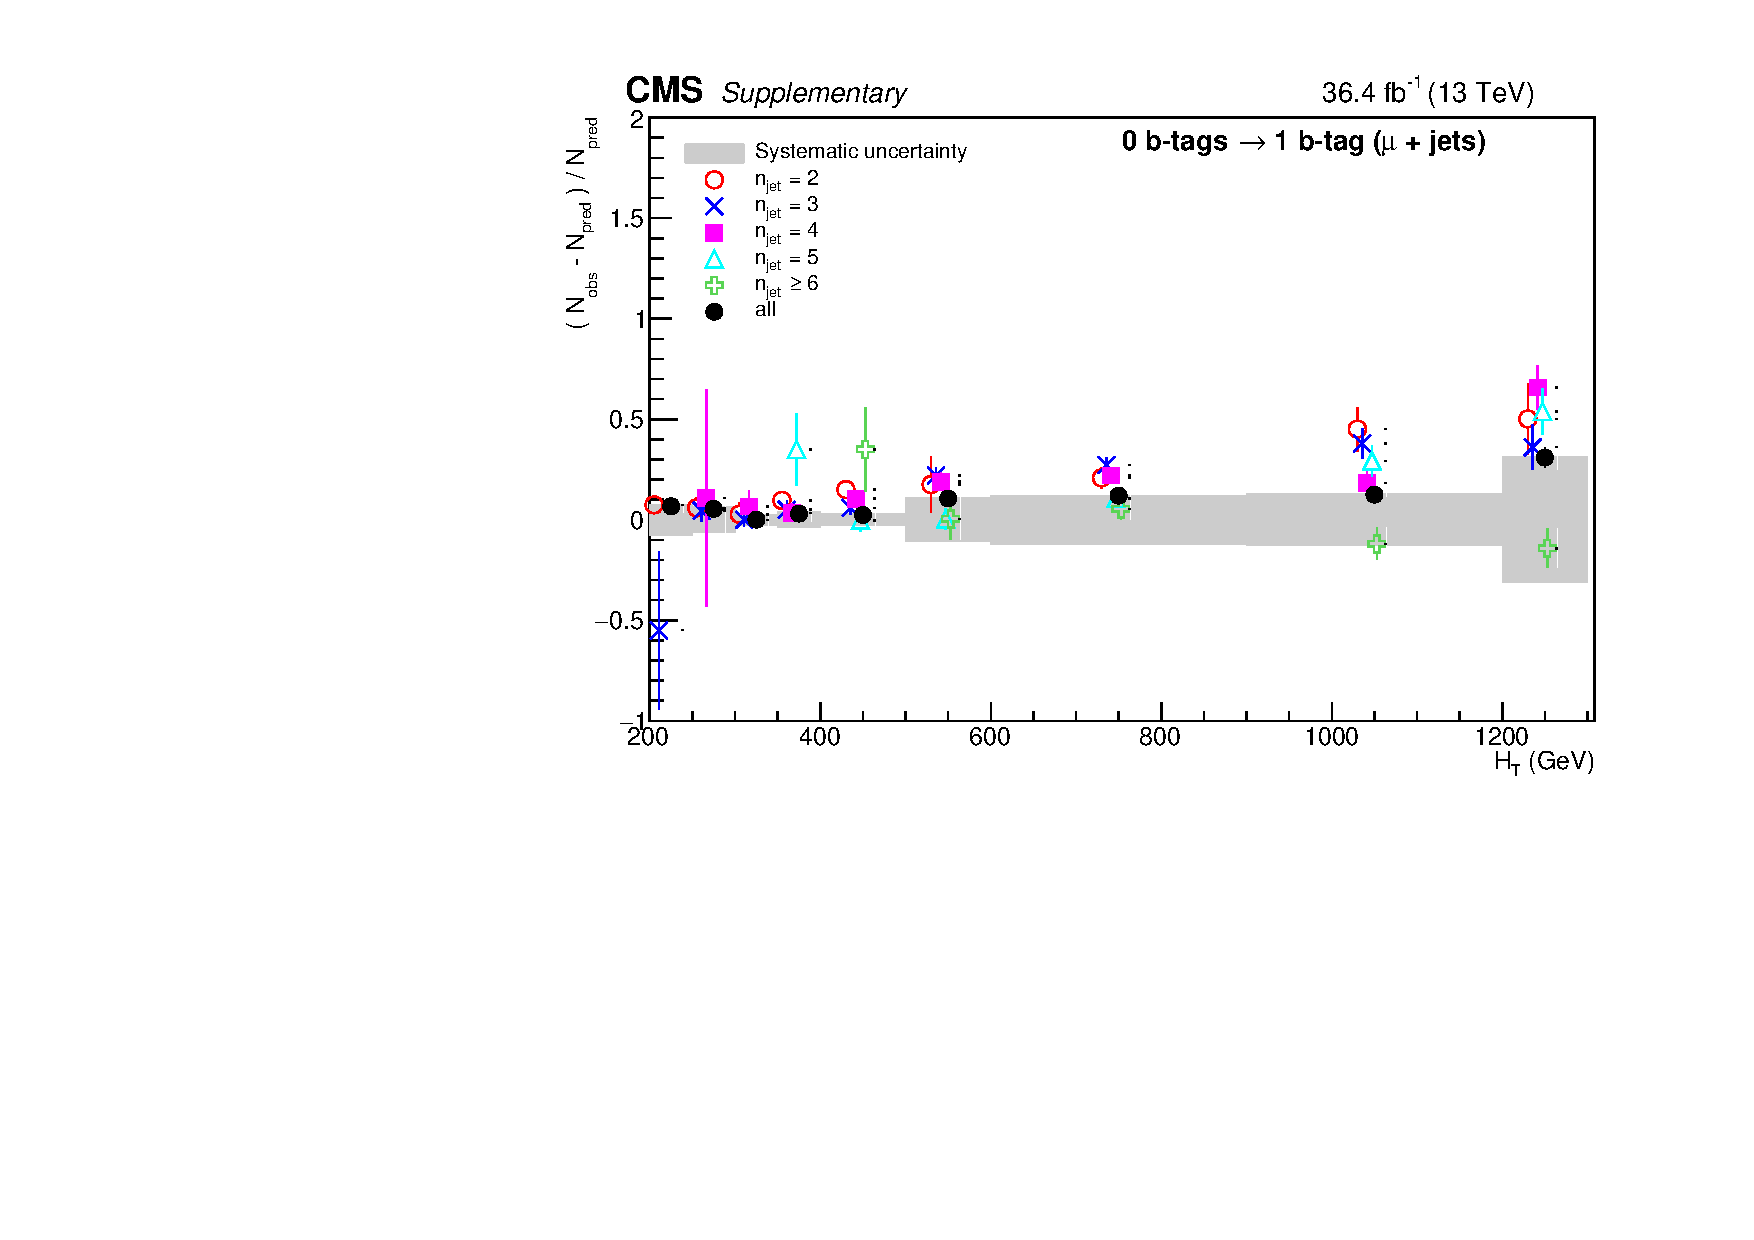
\includegraphics[width=0.5\textwidth]{figures/closureTests/eq0b_eq1b_muon_sym__noFit.pdf}}
    ~~
    \subfigure[]{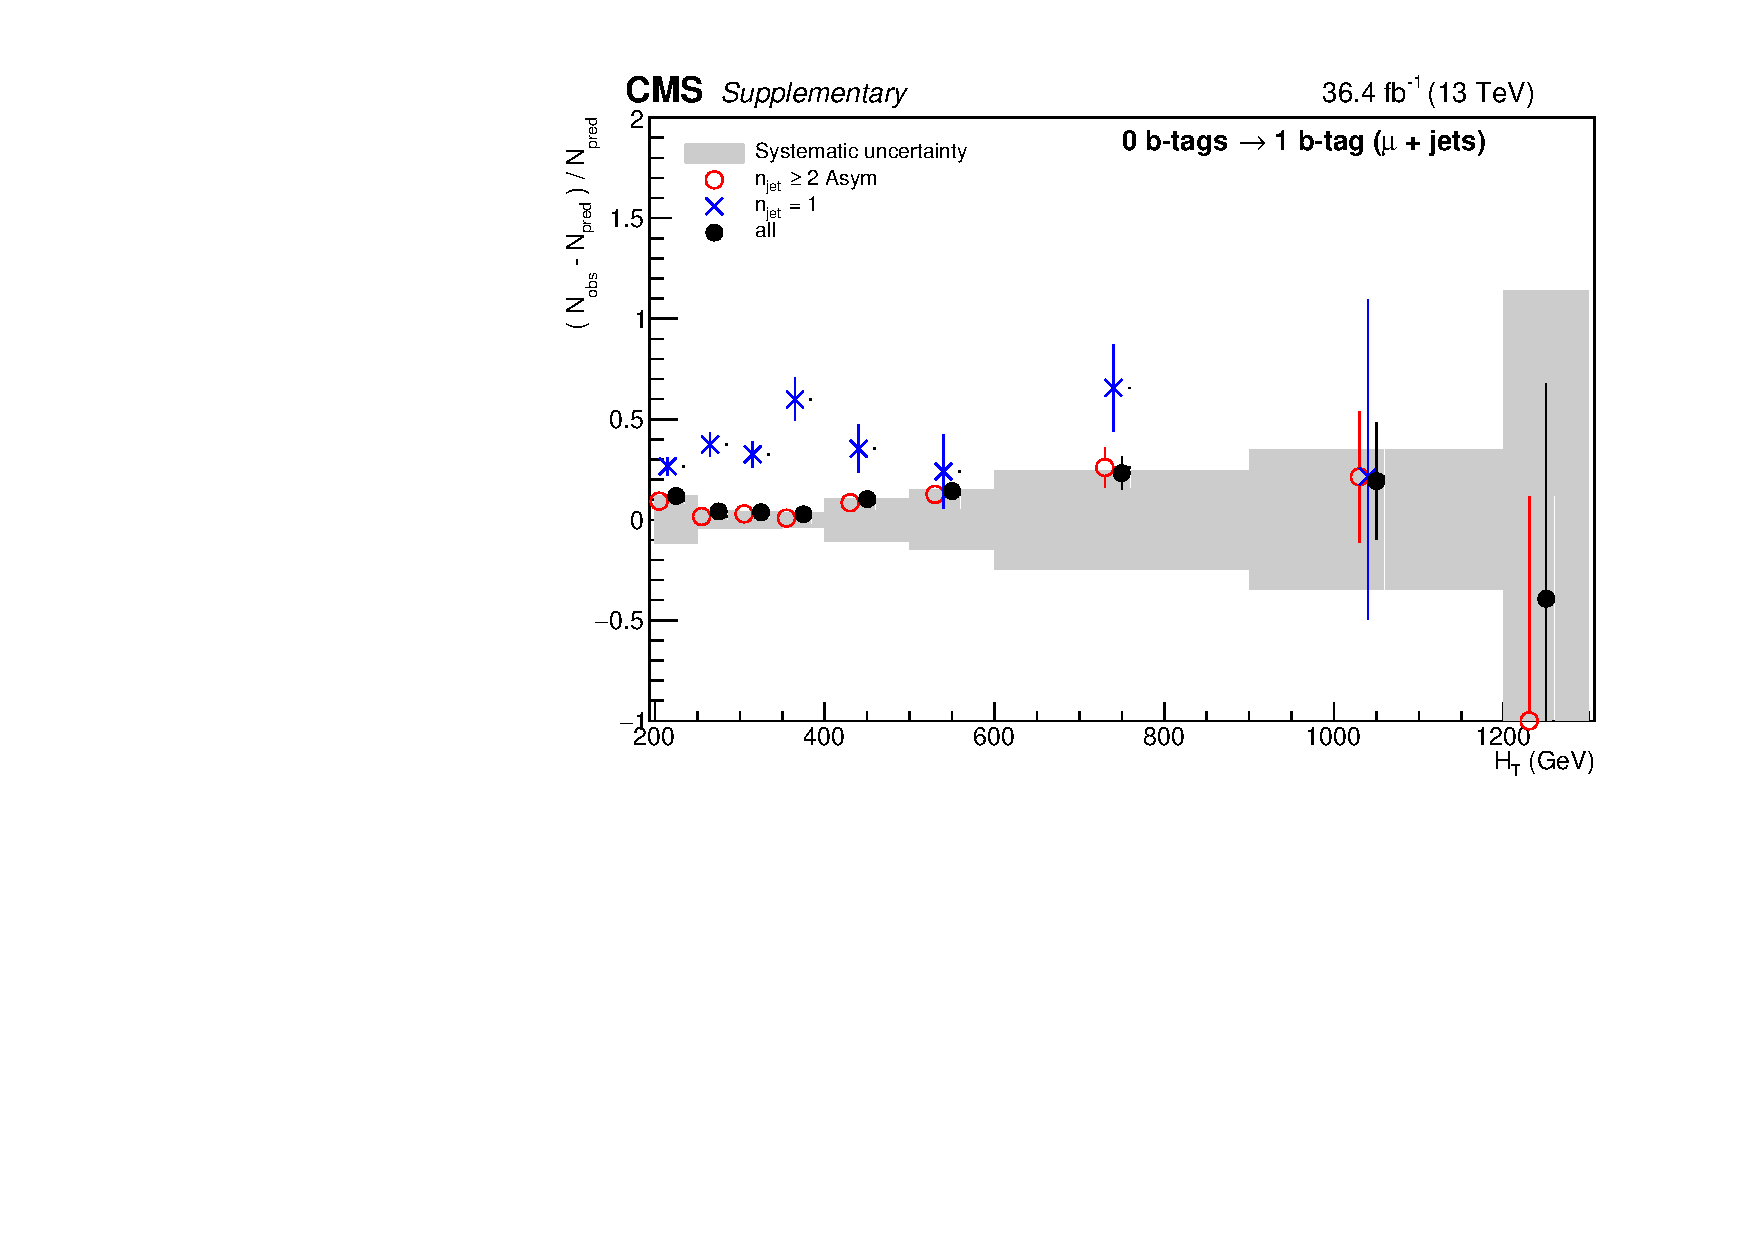
\includegraphics[width=0.5\textwidth]{figures/closureTests/eq0b_eq1b_muon_asym__noFit.pdf}} 
    \caption{Data-driven tests probing the W and \ttbar admixture in
      each \njet category (open symbols). The symmetric (asymmetric)
      jet topologies are shown in the left (right) plot. The BTV POG
      b-tag SFs and their uncertainties are applied in the analysis,
      discussed in Section~\ref{sec:inputs-and-updates}, thus the
      derived systematic is not propagated to the fit. Instead this 
      closure tests is inspected solely as a cross-check. 
    }
    \label{fig:closureBTag}
  \end{center} 
\end{figure}

\newpage
\begin{landscape}
\begin{table}[h!]
  \caption{Summary of the systematics on the transfer factors considered in the analysis, 
    with representatives ranges of uncertainties and the correlation assumed, 
    for the predictions of the $\ttbar$, W and $\znunu$  background
    components.}
  \label{tab:systs}
  \centering
  \scriptsize
  \begin{tabular}{ ccccccc }
    \hline
    \hline
    Systematic & Method & \multicolumn{4}{c}{Relative uncertainty on transfer factor} & Correlation model \\    
    & & $\mj \rightarrow \znunu$  & $\mmj \rightarrow \znunu$ & $\gj \rightarrow \znunu$ & $\mj \rightarrow \ttbar+W$ & \\
    \hline
    Jet energy scale                  & MC variations     & $1-5\%$  & $1-5\%$  & $1-5\%$  & $1-5\%$  & fully correlated                      \\
    B-tagging efficiency b and c jets & MC variations     & $1-3\%$  & $1-3\%$  & $1-3\%$  & $1-3\%$  & fully correlated                      \\
    B-tagging efficiency light jets   & MC variations     & $1-3\%$  & $1-3\%$  & $1-3\%$  & $1-3\%$  & fully correlated                      \\
    Pileup weights                    & MC variations     & $1-7\%$  & $1-7\%$  & $1-7\%$  & $1-7\%$  & fully correlated                      \\
    %Top $p_{T}$ weights              & MC variations     & $1-30\%$ & $1-10\%$ & -        & $1-10\%$ & fully correlated                      \\
    Lepton scale factor               & MC variations     & $1-3\%$  & $1-3\%$  & -        & $1-3\%$  & fully correlated                      \\
    Signal trigger efficiency         & MC variations     & $1-7\%$  & $1-7\%$  & $1-7\%$  & $1-7\%$  & fully correlated                      \\
    %Photon trigger efficiency        & MC variations     & -        & -        & $1-2\%$  & -        & fully correlated                      \\
    \hline
    \alphat/\bdphi extrapolation      & data-driven tests & $3-20\%$ & $3-20\%$ & -        & $3-20\%$ & un-correlated across \scalht/jet top. \\
    W/Z ratio                         & data-driven tests & $1-12\%$ & -        & -        & -        & un-correlated across \scalht/jet top. \\
    Z/$\gamma$ ratio                  & data-driven tests & -        & -        & $2-26\%$ & -        & un-correlated across \scalht/jet top. \\
    W polarisation                    & data-driven tests & $2-14\%$ & -        & -        & $2-14\%$ & un-correlated across \scalht/jet top. \\
    \hline
    \hline
  \end{tabular}
\end{table}

\end{landscape}
